% !TEX root = ../main.tex



\bigskip
\chapter{Vigra Graph Library} \label{ch:vigra_graph_lib}

Vigra \cite{software_vigra} is library for image processing and analysis.
Vigra provides customizable and genric algorithms and datastructures.
Vigra is capable of dealing with multi-dimensional images 
and many algorithms are implemented for arbitrary data types
and dimensions.
Vigra has a wide range of features from simple convolution filters, 
tensor based image processing to machine learning algorithms 
as decision trees.

To simplify the implementation of algorithms for images arbitrary 
dimension, vigra uses a grid graph which is capable of
dealing with any dimension.

Within this thesis we extend the concept graph based image processing
within vigra w.r.t. graphs of any structure.
We put main emphasis on extendability while keeping the usage very simple.


\section{Graph API's}\label{sec:graph_apis}

We strongly belief is is beneficial to use an existing API's for
graphs instead of inventing an own graph API for Vigra.
Coming up with a new API is not straight forward
since one might to think of any future use case this API.
In addition, users became accustomed with existing API's as 
the LEMON or Boost graph API.
Existing algorithms of a particular API can be reused if we stick
to that API.




\subsection{LEMON Graph API's}\label{sec:lemon_graph_apis}
    LEMON \citet{ software_lemon} 
    stand for  ``Library for Efficient Modeling and Optimization in Networks.''.
    It is an open source C++ library with algorithms and data structures 
    related to directed and undirected graphs.
    The extensive usage of templates make this library very flexible.
    While lemon provides a huge set of graph algorithms,
    we are mostly interested in the graph API itself.
    In the following we will give a brief overview of lemons graph 
    API and the related concepts.
    Explaining the complete lemon graph API in detail
    is beyond the scope of this thesis.
    Interested readers are referred to \citet{software_lemon}.
    We will only discuss the API for undirected graphs since any
    graph algorithm we implemented within this thesis
    will work on undirected graphs.

\subsubsection{Graph Items}
    Any undirected graph class fulfilling the lemon API needs to define 
    the following \emph{descriptor} types to represent the graph items.
    \begin{compactitem}
    \item \lstinline{Graph::Edge}
    \item \lstinline{Graph::Arc}
    \item \lstinline{Graph::Node}
    \end{compactitem}
    These \emph{descriptor} should be cheap types which can be copied
    and passed with almost no overhead.
    In addition, descriptor has an unique id
    \footnote{ unique id w.r.t. the item type. 
    Therefore  multiple  nodes cannot have the same id.
    The same holds line for edges and arcs.
    But there might be a node and edge which have the same id}.
    These id's can be accessed via \lstinline{Graph::id(Node)}, \lstinline{Graph::id(Edge)} and \lstinline{Graph::id(Arc)}.
    These id's can not only be dense but also sparse, which is very
    important for an efficient handling of grid graph edge ids.



\subsubsection{Iterators}

    Within lemon a very convenient mechanism is used to iterate over
    nodes, edges and arcs.
    A special constant \lstinline{INVALID} is used to determine if 
    an iterator reached the end.

    \begin{minipage}{\textwidth}\vspace{-0.75cm}\begin{lstlisting}[language=c++]
    // iterate over nodes
    for(Graph::NodeIt v(g); v!= lemon::INVALID; ++v){/*...*/}

    // iterate over edges
    for(Graph::EdgeIt e(g); e!= lemon::INVALID; ++e){/*...*/}

    // iterate over arcs
    for(Graph::ArcIt a(g); a!= lemon::INVALID; ++a){/*...*/}

    // use arcs to iterate over neighbor nodes
    for(Graph::OutArcIt a(g,n); a!= lemon::INVALID; ++a){
        const Node neighborNode = g.target(a);
        /*...*/
    }
    \end{lstlisting}\end{minipage}\vspace{0.5cm}

    Any iterator is convertible to the corresponding item which
    is iterated without using \lstinline{operator*()}.

\subsubsection{Map Concept}

    In lemon, graph classes store only the structure of the graph itself.
    All addition data for nodes, edges and arcs is stored 
    in \emph{maps}. 
    Any graph has default implementations for graph maps which
    can be accessed in the following way.

    \begin{minipage}{\textwidth}\vspace{-0.75cm}\begin{lstlisting}[language=c++]
    // edge map (for data as edge weights)
    Graph::EdgeMap<float> edgeMap(g); 

    // read and write data 
    for(Graph::EdgeIt e(g); e!= lemon::INVALID; ++e){
        // read
        const float val = edgeMap[*e];
        // write
        edgeMap[*e] = std::exp(-1.0*a);
    }

    // node map (for node related data as node labelings )
    Graph::NodeMap<usigned int> nodeMap(g);
    for(Graph::NodeIt v(g); v!= lemon::INVALID; ++v){
        // read
        const unsigned int val = nodeMap[*e];
        // write
        nodeMap[*e] = val+1;
    }
    \end{lstlisting}\end{minipage}\vspace{0.5cm}


    Custom maps can be implemented very easy:

    \begin{minipage}{\textwidth}\vspace{-0.75cm}\begin{lstlisting}[language=c++]
    template<class Graph>
    class ImplicitEdgeMap {
    public:
        typedef typename Graph::Edge Key;
        typedef double Value;
        Value operator[](Key edge) const { 
            Value a;
            /*...*/
            return a;
        }
    };
    \end{lstlisting}\end{minipage}\vspace{0.5cm}

\subsection{BOOST Graph API's}\label{sec:boost_graph_apis}
The Boost Graph Library (BGL)  \cite{software_bgl} is set of data structures and 
algorithms for graph related computations.
Since all algorithms are implemented within the LEMON graph interface, 
the BGL graph API will only be described briefly.
The graph API defined in the BGL is a collection of
free functions and graph traits which can be specialized for
any graph.




\subsection{VIGRA Graph API}

While the grid graph is implemented within the BGL and LEMON graph API,\
all algorithms implemented within this thesis will
use the LEMON graph API instead of the BGL 
for the following reason.
\todo{write reasons...}





\section{Implementation}\label{sec:vigra_graph_lib_impl}

The most important concept for graph based image processing
is the \emph{region adjacency graph} (RAG) (see \cref{fig:make_rag}).

A RAG is extracted from a labeled \emph{base graph}.
In the first step of graph based image processing, the base 
graph is usually a grid graph, and the labeling is a label image
as in \cref{fig:make_rag} .
To encode a RAG we need a undirected graph, 
and a mapping from the base graphs edges and nodes to the RAG 
needs to be stored.

The implementation of grid graphs is explained in \cref{sec:graphs_grid_graph}, 
a basic undirected graphs implementation will be discussed in \cref{sec:graphs_adjacency_list_graph}.
The implementation details of the \emph{region adjacency graph} concept will 
be given in  \cref{sec:graphs_rag}.

For hierarchical clustering we provide a specialized graph, named \emph{merge graph}.


To implemented structured clustering algorithms (see \cref{sec:rw_hc} we
need a graph which supports the contraction of edges.
Also a mechanism to merge node and edge features is needed.
Within \cref{sec:graphs_merge_graph} we propose  a very flexible
and concept for hierarchical clustering based on a specialized graph,
called \emph{merge graph}.


A generic set of algorithms which work on any graph
implemented within the VIGRA graph api is presented 
in \cref{sec:graph_graph_algorithms}.

While the core implementation of any algorithm is in C++
VIGRA provides python binding to make almost
any algorithm available in Python.
To provide a generic Python interface for any proposed
graph, we need to introduce a few concepts 
to make the python wrapped graph API very \emph{Pythonic}


\subsection{Graphs}


\subsubsection{Grid Graph} \label{sec:graphs_grid_graph}

\missingfigure{show grid graph here}

    \lstinline{vigra::GridGraph<DIM,DIRECTED_TAG>}

\subsubsection{Adjacency List Graph} \label{sec:graphs_adjacency_list_graph}


    \begin{minipage}{\textwidth}\vspace{-0.75cm}\begin{lstlisting}[language=c++]
    typedef AdjacencyListGraph Graph;

    // construct graph
    Graph g;

    // add nodes (id will be asigned automatically)
    Graph::Node n0 = g.addNode() 

    // add node with an explicit id
    Graph::Node n3 = g.addNode(3)

    // add edges from existing nodes
    Graph::Edge e0 = g.addEdge(n0,n1)

    // add edges and nodes simultaneous 
    Graph::Edge e1 = g.addEdge(2,3)

    // no parallel edges 
    Graph::Edge e2 = g.addEdge(2,3)
    assert(e1==e2)  
    \end{lstlisting}\end{minipage}\vspace{0.5cm}



\subsubsection{Region Adjacency Graph} \label{sec:graphs_rag}

To get a region adjacency graph (RAG), a labeled graph is needed.
The labeled graph will hereinafter be referred to as \emph{base graph} 
$G_{\text{base}}$
of the RAG.

To map edges and nodes from the base graph


\subsubsection{Merge Graph} \label{sec:graphs_merge_graph}
To implemented structured clustering algorithms (see \cref{???}) we
need a graph which supports the contraction of edges.
Also a mechanism to merge node and edge features is needed.
Experiments suggest that the edge contraction is more expensive
than feature merging an can even be a bottleneck for huge 3D data 
(see \cref{???} ).
Therefore it is crucial to implemented the MergeGraph (MG) very carefully.
\begin{figure}
    \centering
    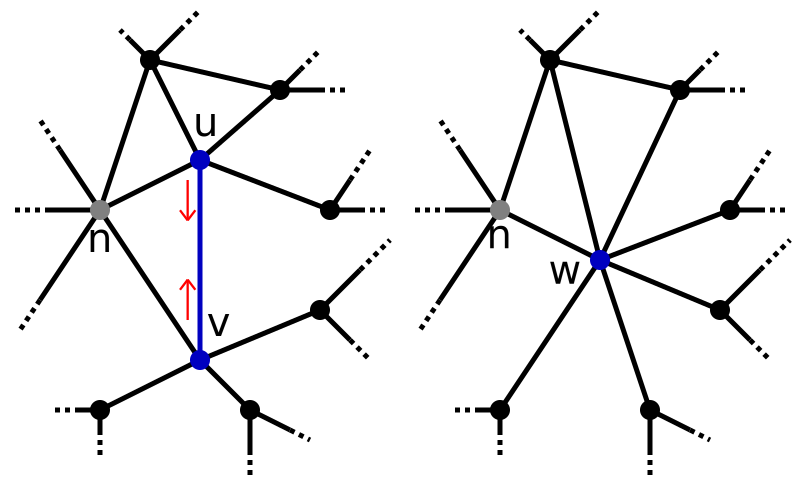
\includegraphics[width=0.35\textwidth]{fig/contraction.pdf}

    \addtocontents{lof}{%
        \vspace{1cm}
        \protect\centerline{%
            \protect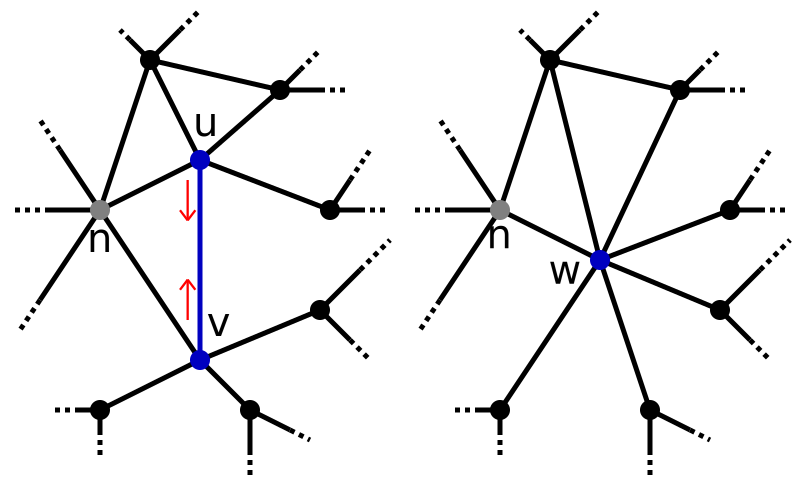
\includegraphics[width=\lofthumbsize,height=\lofthumbsize,keepaspectratio=true]{fig/contraction.pdf} 
        } 
    }%

    %\addtocontents{lof}{%
    %    $\vcenter to \lofthumbsize{\vss%
    %        \hbox to \lofthumbsize {
    %            \hss \protect 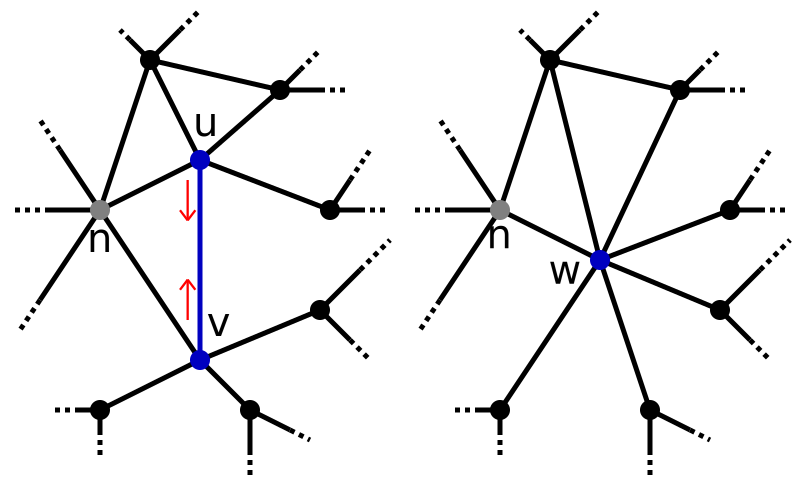
\includegraphics[width=.075\linewidth]{fig/contraction.pdf} \hss
    %        }
    %    \vss}$%
    %    \quad
    %    \ignorespaces
    %}%
    \caption[Schematic edge contraction]{ Schematic edge contraction: Node $u$ and $v$ is merged into node $w$.
        Note the gray node $n$ which is connected to $u$ and $v$.
        After the contraction, edges $\{ n,u\}$ and $\{ n,v\}$ are also merged into 
        a single edge $\{ n, w\}$ 
    }
    \label{fig:figlabel}
\end{figure}


   

\begin{center}
    \begin{tikzpicture}
        \umlclass[template=Graph]{MergeGraphAdpator}
        {
            \\// union find data structures                     \\
            - edgeUfd               : IterablePartiton          \\
            - nodeUfd               : IterablePartiton          \\ 
            - nodesAdjacency        : AdjacencySetVector        \\

            \\// callbacks                                      \\
            - mergeNodeCallBacks    : MergeNodeCallBackVector   \\
            - mergeEdgeCallBack     : MergeEdgeCallBackVector   \\
            - eraseEdgeCallBack     : EraseEdgeCallBackVector   \\
        }
        {
            \\// LEMON API for undirected graphs                \\
                $\ldots$                                        \\
            \\// register callbacks                             \\ 
            + registerMergeNodeCallBack(f : MergeNodeCallBack)  \\
            + registerMergeEdgeCallBack(f : MergeEdgeCallBack)  \\
            + registerEraseEdgeCallBack(f : EraseEdgeCallBack)  \\

            \\// modify graph                                   \\
            + contractEdge(edge : Edge)     : Node              \\

            \\// find representatives                           \\
            + reprNode(node : Node)         : Node              \\
            + reprEdge(edge : Edge)         : Edge              \\ 

            \\// get base graph                                 \\
            + graph()                       : Graph             \\
        } 
    \end{tikzpicture}
\end{center}

\begin{center}
    \begin{tikzpicture}
        \umlclass[template=MergeGraph]{ClusterOperatorInterface}
        {

        }
        {
            \\// contract next edge and get weight              \\
            + contractionEdge(edge : Edge)         : Edge       \\ 
            + contractionWeight(edge : Edge)       : Edge       \\
            \\// get base graph                                 \\
            + mergeGraph()                  : MergeGraph        \\
        } 
    \end{tikzpicture}
\end{center}

\begin{center}
    \begin{tikzpicture}
        \umlclass[template=ClusterOperator]{HierarchicalClustering}
        {

        }
        {
            + cluster()                     : void        \\
            + reprLabels(nodeMap : NodeMap) : void        \\      
        } 
    \end{tikzpicture}
\end{center}


   We propose and implemented the following design:
   \begin{compactitem}
       \item  A base graph is attached to a merge graph  and  a merge graph will
            always ``view'' to
       \item  Union find data structure for nodes
       \item  Union find data structure for edges
   \end{compactitem}



   \lstinline{vigra::MergeGraphAdaptor<DIM,DIRECTED_TAG>}


\subsection{Graph Algorithms} \label{sec:graph_graph_algorithms}

    \subsubsection{Multicut}

    \subsubsection{Hierarchical Clustering}

    \subsubsection{Mst Algorithms}

    \subsubsection{Watershed Algorithms}

    \subsubsection{Smoothing Algorithms}





\section{Python}




\begin{flushright}{\slshape    
(1) Beautiful is better than ugly. \\ \label{cit:line_a}
(2) Explicit is better than implicit. \\ \label{cit:line_b}
(3) Simple is better than complex. \\
(4) Complex is better than complicated. \\
(5) Flat is better than nested. \\
(6) Sparse is better than dense. \\
(7) Readability counts. \\
(8) Special cases aren't special enough to break the rules. \\
(9) Although practicality beats purity. \\
(10) Errors should never pass silently. \\
(11) Unless explicitly silenced. \\
(12) In the face of ambiguity, refuse the temptation to guess. \\
(13) There should be one-- and preferably only one --obvious way to do it. \\
(14) Although that way may not be obvious at first unless you're Dutch. \\
(15) Now is better than never. \\
(16) Although never is often better than *right* now. \\
(17) If the implementation is hard to explain, it's a bad idea. \\
(18) If the implementation is easy to explain, it may be a good idea. \\
(19) Namespaces are one honking great idea -- let's do more of those! } \\ \medskip
--- The Zen of Python
\end{flushright}
\captionof{figure}{ 
    The Zen of Python
}\label{fig:zen_of_python}






\subsection{Graph Maps}

On the python side, we want node-maps, edge-maps and arc-maps to be stored 
as numpy arrays for several reasons.
Numpy arrays are the standard for storing multidimensional data in python.
The fast C implementation and the highly vectorized API of numpy makes it very easy to write 
fast python code within a few lines.
Virtually any python user will be familiar with the numpy API and therefore it 
seems to be natural to store graph maps within numpy arrays.

In addition VIGRA provides an mechanism to pass numpy arrays to C++.
Therefore no new mechanism needs to be implemented to transfer graph
maps from python to C++.
This will not only simplify writing extension for the new VIGRA graph API,
but also it will reduce the glue code since we can use well tested existing
solutions.

New algorithms might be implemented in pure python with a mix of
existing numpy functions and new functions provided within VIGRA's graph API.
As a proof of concept we implemented ??? in pure python with VIGRA's
fresh graph API in \cref{???}.


\subsubsection{Intrinsic Graph Shape}

Each graph has an \emph{intrinsic node map shape} 
and an \emph{intrinsic edge map shape} and 
These intrinsic shape and dimensions are used to use 
numpy arrays with the best fitting dimension and shape.
For a 2D grid graph the node map should also be a 2D dimensional array.
because in this way an usual image can be used as an node map.
To access the  intrinsic shapes of node and edge maps 
we use a small trait class with default implementations
for unknown graphs.
The default implementation is given below:

\begin{minipage}{\textwidth}\vspace{-0.75cm}\begin{lstlisting}[language=c++]
template<class GRAPH>
class IntrinsicGraphShape{
private:
    typedef GRAPH Graph;
    typedef typename vigra::MultiArray<1,int>::difference_type DiffType1d;
    typedef typename Graph::index_type  index_type;
public:
    typedef typename Graph::Node Node ;
    typedef typename Graph::Edge Edge ;
    typedef typename  Graph::Arc  Arc ;

    typedef DiffType1d IntrinsicNodeMapShape;
    typedef DiffType1d IntrinsicEdgeMapShape;
    typedef DiffType1d  IntrinsicArcMapShape;

    static IntrinsicNodeMapShape intrinsicNodeMapShape(const Graph & g){
        return IntrinsicNodeMapShape(g.maxNodeId()+1);
    }
    static IntrinsicEdgeMapShape intrinsicEdgeMapShape(const Graph & g){
        return IntrinsicEdgeMapShape(g.maxEdgeId()+1);
    }
    static IntrinsicArcMapShape intrinsicArcMapShape(const Graph & g){
        return  IntrinsicArcMapShape(g.maxArcId()+1);
    }

    static const unsigned int IntrinsicNodeMapDimension=1;
    static const unsigned int IntrinsicEdgeMapDimension=1;
    static const unsigned int IntrinsicArceMapDimension=1;
};
\end{lstlisting}\end{minipage}\vspace{0.5cm}



\subsubsection{Numpy Arrays To LEMON Maps}


On the C++ side, numpy arrays are stored in MultiArrayViews.
Since the API of MultiArrayViews \cite{software_vigra_multiarray_api} does
not implemented the API  of LEMON graph maps (e.g. node-maps, edge-maps and arc-maps), 
a thin wrapper is used to convert the arrays to LEMON conform maps.
These wrappers can be accessed via \lstinline{PyNodeMapTraits<Graph,T>::Array} and 
\lstinline{PyNodeMapTraits<Graph,T>::Map}. 


In the following we will give a brief example how to pass numpy arrays to C++
and convert them to LEMON conform graph maps.

Assuming we need a function which does something with node features as normalization.
On the python side we want to have the following signature:

\lstinline{result=vigra.graphs.normNodeFeat(graph,nodeFeatures=nodeFeatures,out=None)}.

The function should work on single band node features and multi band node features
(an arbitrary number of channels, but the same for all nodes).
There should be a single C++ function which can be used to export
\lstinline{normNodeFeat} for any graph within VIGRA's graph API. 




\begin{minipage}{\textwidth}

To archive this we propose the following design:
On the C++ side we use a function  which
is has two templates , one for the graph, and one for the value type.
A prototypical implementation is given below.

\begin{minipage}{\textwidth}\vspace{-0.75cm}\begin{lstlisting}[language=c++]
template<class Graph,class T>
NumpyAnyArray normNodeFeat(
    const Graph & g,
    const typename PyNodeMapTraits<Graph,T >::Array & nodeFeaturesInArray,
    typename PyNodeMapTraits<Graph,T>::Array  outArray 
){
    // reshape out 
    // - last argument (outArray) will be reshaped if empty,
    // - and #channels is taken from second argument (nodeFeaturesIn) 
    reshapeNodeMapIfEmpty(g,nodeFeaturesIn,outArray);

    // numpy arrays => lemon maps 
    // featuresInMap and outMap fulfill
    // the concept of LEMON NODE MAPS
    typename PyNodeMapTraits<Graph,T >::Map featuresInMap(g,nodeFeaturesInArray);
    typename PyNodeMapTraits<Graph,T >::Map outMap(g,outArray);


    /* call code using LEMON API*/

    // return out as numpy array
    return outArray;
}
\end{lstlisting}\end{minipage}\vspace{0.5cm}

The template \lstinline{T} can be instantiated with scalars as \lstinline{float}, an explicit single band scalar as \lstinline{Singleband<float>}
or a multi band type as \lstinline{Multiband<float>}.

\lstinline{PyNodeMapTraits<Graph,T >::Array} will select the correct \lstinline{vigra::NumpyArray<DIM,VALUE_TYPE>} w.r.t.
the templates \lstinline{Graph} and \lstinline{T}.

The output array will be reshaped with the corrected number of channels by calling \lstinline{reshapeNodeMapIfEmpty}.
Equivalent functions exist for edge maps.

\lstinline{PyNodeMapTraits<Graph,T >::Map} is the corresponding LEMON conform  node map 
which is a cheap view to an numpy array. 
\end{minipage}


\begin{minipage}{\textwidth}
To make the function above available in python
we need to write wrapper code with \lstinline{boost::python}.
We will export the function for single band floats and multi band floats.

\begin{minipage}{\textwidth}\vspace{-0.75cm}\begin{lstlisting}[language=c++]
// single-band float32
boost::python::def(
    "normNodeFeat",
     &normNodeFeat<Graph,float>,
    (
        boost::python::arg("graph"),
        boost::python::arg("nodeFeatures"),
        boost::python::arg("out")=boost::python::object() // None
    )
);

// multi-band float32
boost::python::def(
    "normNodeFeat",
     &normNodeFeat<Graph,Multiband<float> >,
    (
        boost::python::arg("graph"),
        boost::python::arg("nodeFeatures"),
        boost::python::arg("out")=boost::python::object() // None
    )
);
\end{lstlisting}\end{minipage}\vspace{0.5cm}

\end{minipage}


On the python side we can call the function as desired.
The array which stores the result of this
function can be preallocated and passed explicitly.

\begin{minipage}{\textwidth}\vspace{-0.75cm}\begin{lstlisting}[language=Python]
// with automatically allocated outFeatures
outFeatures = vigra.graphs.normNodeFeat(graph,nodeFeatures)

// with explicitly given outFeatures
// - here we assume single band features
outFeatures2 = vigra.graphs.graphMap(graph,item='node',dtype=np.float32)
outFeatures2 = vigra.graphs.normNodeFeat(graph,nodeFeatures,out=outFeatures2)


// with multiband node features 
// - here we assume multi band features
//   with 3 channels per node
outFeatures2 = vigra.graphs.graphMap(graph,item='node',dtype=np.float32,channels=3)
outFeatures2 = vigra.graphs.normNodeFeat(graph,nodeFeatures,out=outFeatures2)
\end{lstlisting}\end{minipage}\vspace{0.5cm}




\subsection{Graph Hierarchy}
    
Explain the very nice workflow 